% Options for packages loaded elsewhere
\PassOptionsToPackage{unicode}{hyperref}
\PassOptionsToPackage{hyphens}{url}
%
\documentclass[a4paper,DIV=11
%headsepline
]{scrartcl}


%\usepackage[a4paper, left=2.5cm, right=2.5cm,top=2cm, bottom=2cm, includehead, includefoot, headsep=.8cm, footskip=1cm]{geometry}


% Beseitigt ein paar Fehlermeldungen in KOMA-Script, bezüglich der Notenbeispiel-Verzeichnisse
\usepackage{scrhack}

\usepackage{xcolor}

\usepackage{scrlayer-scrpage}
%\clearpairofpagestyles
\cfoot{\pagemark}
\chead{\headmark}
\automark{section}
\pagestyle{headings}

\usepackage{mdwlist}

%\setkomafont{pagenumber}{\small}

%% Engere Variante! Spart Platz
\usepackage{tgpagella}
\usepackage{tgheros}
%% Sieht schöner aus als courier
\usepackage[scaled=.95]{sourcecodepro}
%\usepackage[osf]{mathpazo}
%\usepackage[scaled=.95]{helvet}
%\usepackage{courier}


\usepackage[ngerman]{babel}
%\usepackage{amsmath,amssymb}
%\usepackage{lmodern}
\usepackage{iftex}
\ifPDFTeX
  \usepackage[T1]{fontenc}
  \usepackage{textcomp} % provide euro and other symbols
\else % if luatex or xetex
  \usepackage{unicode-math}
  \defaultfontfeatures{Scale=MatchLowercase}
  \defaultfontfeatures[\rmfamily]{Ligatures=TeX,Scale=1}
\fi
% Use upquote if available, for straight quotes in verbatim environments
\IfFileExists{upquote.sty}{\usepackage{upquote}}{}
\IfFileExists{microtype.sty}{% use microtype if available
  \usepackage[]{microtype}
  \UseMicrotypeSet[protrusion]{basicmath} % disable protrusion for tt fonts
}{}
\makeatletter
\@ifundefined{KOMAClassName}{% if non-KOMA class
  \IfFileExists{parskip.sty}{%
    \usepackage{parskip}
  }{% else
    \setlength{\parindent}{0pt}
    \setlength{\parskip}{6pt plus 2pt minus 1pt}}
}{% if KOMA class
  }
\makeatother
\newcommand{\computer}[1]{\texttt{#1}}
\usepackage{xcolor}
\usepackage{color}
\usepackage{fancyvrb}
\newcommand{\VerbBar}{|}
\newcommand{\VERB}{\Verb[commandchars=\\\{\}]}
\DefineVerbatimEnvironment{Highlighting}{Verbatim}{commandchars=\\\{\}}
% Add ',fontsize=\small' for more characters per line
\newenvironment{Shaded}{}{}
\newcommand{\AlertTok}[1]{\textcolor[rgb]{1.00,0.00,0.00}{\textbf{#1}}}
\newcommand{\AnnotationTok}[1]{\textcolor[rgb]{0.38,0.63,0.69}{\textbf{\textit{#1}}}}
\newcommand{\AttributeTok}[1]{\textcolor[rgb]{0.49,0.56,0.16}{#1}}
\newcommand{\BaseNTok}[1]{\textcolor[rgb]{0.25,0.63,0.44}{#1}}
\newcommand{\BuiltInTok}[1]{\textcolor[rgb]{0.00,0.50,0.00}{#1}}
\newcommand{\CharTok}[1]{\textcolor[rgb]{0.25,0.44,0.63}{#1}}
\newcommand{\CommentTok}[1]{\textcolor[rgb]{0.38,0.63,0.69}{\textit{#1}}}
\newcommand{\CommentVarTok}[1]{\textcolor[rgb]{0.38,0.63,0.69}{\textbf{\textit{#1}}}}
\newcommand{\ConstantTok}[1]{\textcolor[rgb]{0.53,0.00,0.00}{#1}}
\newcommand{\ControlFlowTok}[1]{\textcolor[rgb]{0.00,0.44,0.13}{\textbf{#1}}}
\newcommand{\DataTypeTok}[1]{\textcolor[rgb]{0.56,0.13,0.00}{#1}}
\newcommand{\DecValTok}[1]{\textcolor[rgb]{0.25,0.63,0.44}{#1}}
\newcommand{\DocumentationTok}[1]{\textcolor[rgb]{0.73,0.13,0.13}{\textit{#1}}}
\newcommand{\ErrorTok}[1]{\textcolor[rgb]{1.00,0.00,0.00}{\textbf{#1}}}
\newcommand{\ExtensionTok}[1]{#1}
\newcommand{\FloatTok}[1]{\textcolor[rgb]{0.25,0.63,0.44}{#1}}
\newcommand{\FunctionTok}[1]{\textcolor[rgb]{0.02,0.16,0.49}{#1}}
\newcommand{\ImportTok}[1]{\textcolor[rgb]{0.00,0.50,0.00}{\textbf{#1}}}
\newcommand{\InformationTok}[1]{\textcolor[rgb]{0.38,0.63,0.69}{\textbf{\textit{#1}}}}
\newcommand{\KeywordTok}[1]{\textcolor[rgb]{0.00,0.44,0.13}{\textbf{#1}}}
\newcommand{\NormalTok}[1]{#1}
\newcommand{\OperatorTok}[1]{\textcolor[rgb]{0.40,0.40,0.40}{#1}}
\newcommand{\OtherTok}[1]{\textcolor[rgb]{0.00,0.44,0.13}{#1}}
\newcommand{\PreprocessorTok}[1]{\textcolor[rgb]{0.74,0.48,0.00}{#1}}
\newcommand{\RegionMarkerTok}[1]{#1}
\newcommand{\SpecialCharTok}[1]{\textcolor[rgb]{0.25,0.44,0.63}{#1}}
\newcommand{\SpecialStringTok}[1]{\textcolor[rgb]{0.73,0.40,0.53}{#1}}
\newcommand{\StringTok}[1]{\textcolor[rgb]{0.25,0.44,0.63}{#1}}
\newcommand{\VariableTok}[1]{\textcolor[rgb]{0.10,0.09,0.49}{#1}}
\newcommand{\VerbatimStringTok}[1]{\textcolor[rgb]{0.25,0.44,0.63}{#1}}
\newcommand{\WarningTok}[1]{\textcolor[rgb]{0.38,0.63,0.69}{\textbf{\textit{#1}}}}
\usepackage{graphicx}
\makeatletter
\def\maxwidth{\ifdim\Gin@nat@width>\linewidth\linewidth\else\Gin@nat@width\fi}
\def\maxheight{\ifdim\Gin@nat@height>\textheight\textheight\else\Gin@nat@height\fi}
\makeatother
% Scale images if necessary, so that they will not overflow the page
% margins by default, and it is still possible to overwrite the defaults
% using explicit options in \includegraphics[width, height, ...]{}
\setkeys{Gin}{width=\maxwidth,height=\maxheight,keepaspectratio}
% Set default figure placement to htbp
\makeatletter
\def\fps@figure{htbp}
\makeatother
\setlength{\emergencystretch}{3em} % prevent overfull lines
\providecommand{\tightlist}{%
  \setlength{\itemsep}{0pt}\setlength{\parskip}{0pt}}
\setcounter{secnumdepth}{-\maxdimen} % remove section numbering
\ifLuaTeX
  \usepackage{selnolig}  % disable illegal ligatures
\fi
\IfFileExists{bookmark.sty}{\usepackage{bookmark}}{\usepackage{hyperref}}
\IfFileExists{xurl.sty}{\usepackage{xurl}}{} % add URL line breaks if available
\urlstyle{same} % disable monospaced font for URLs
\hypersetup{
  hidelinks,
  pdfcreator={LaTeX via pandoc}}

\author{Manfred Dings}
\title{MAP für Windows}
\subtitle{Ein Mediaplayer für Lehrveranstaltungen}

\begin{document}

\maketitle


\tableofcontents

\hypertarget{map}{%
\section{MAP}\label{map}}

MAP ist ein Programm zum Abspielen von wav- und mp3-Dateien, gekoppelt
mit Kommentaren, Hinweistexten oder Höraufgaben, die nach einer
bestimmten Zeitvorgabe gestartet werden. Die Hinweistexte können
zusammen mit einer Uhr in einem zweiten Programmfenster dargestellt
werden, das bei Bedarf auf einen zweiten Bildschirm geschoben werden
kann und dort als "`always on top"'-Fenster über weiteren Inhalten (z.
B. einer Präsentation) dargestellt werden kann.

MAP für den Einsatz in Lehrveranstaltungen zur Höranalyse und zur
Präsentation von Musikbeispielen in Vorlesungen und dergleichen
entwickelt.

Die Benutzung von MAP geschieht auf eigene Gefahr. © 2016 by Manfred
Dings. MAP ist unter LGP lizensiert. Der Text der LGP ist auf S.~\pageref{lizenz} wiedergegeben.

\hypertarget{programmkonzept-und-erste-schritte}{%
\section{Programmkonzept und erste
Schritte}\label{programmkonzept-und-erste-schritte}}

MAP spielt wie ein üblicher MP3-Player wav- und mp3-Dateien ab
(\protect\hyperlink{FormatSounddateien}{Hinweise zum mp3-Dateiformat}
beachten, siehe S.~\pageref{format-der-sounddateien}). Bei der Wiedergabe läuft eine Uhr mit, zusätzlich lassen sich
Hinweise zu exakt definierbaren Zeitpunkten einblenden. Dazu sind
benötigt das Programm ein abgestuftes System von Dateien: sog.
\protect\hyperlink{aufgabenlisten}{Aufgabenlisten} und
\protect\hyperlink{aufgabendateien}{Aufgabendateien}, beides einfache
Textdateien, die sich in jedem Editor bearbeiten lassen, bei Bedarf auch
\protect\hyperlink{BefehleImMenuAufgabeneditor}{im Programm selber}.
\protect\hyperlink{aufgabenlisten}{Aufgabenlisten} (*.\texttt{afl})
bilden dabei so etwas wie Playlisten. Sie enthalten die Dateinamen von
Aufgabendateien (\texttt{*.auf}), die sich im selben Verzeichnis wie die
Aufgabenliste selbst befinden müssen. Hier ein Beispiel für den Inhalt
einer Aufgabendatei:

	\begin{Shaded}
\begin{Highlighting}[]
\NormalTok{Aufgabe01.auf}
\NormalTok{Aufgabe02.auf}
\NormalTok{Aufgabe03.auf}
\NormalTok{Aufgabe04.auf}
\NormalTok{Aufgabe04a.auf}
\end{Highlighting}
\end{Shaded}

Mit dem Menübefehl \protect\hyperlink{AufgabenlisteLaden}{Aufgabenliste
Laden (F2)} wird eine solche Aufgabenliste eingelesen. Im Listenfeld
links im Programmfenster werden die Beschreibungen der Aufgabendateien
sichtbar und können dort per Menübefehl oder durch Mausklick ausgewählt
werden.

\begin{figure}
\centering
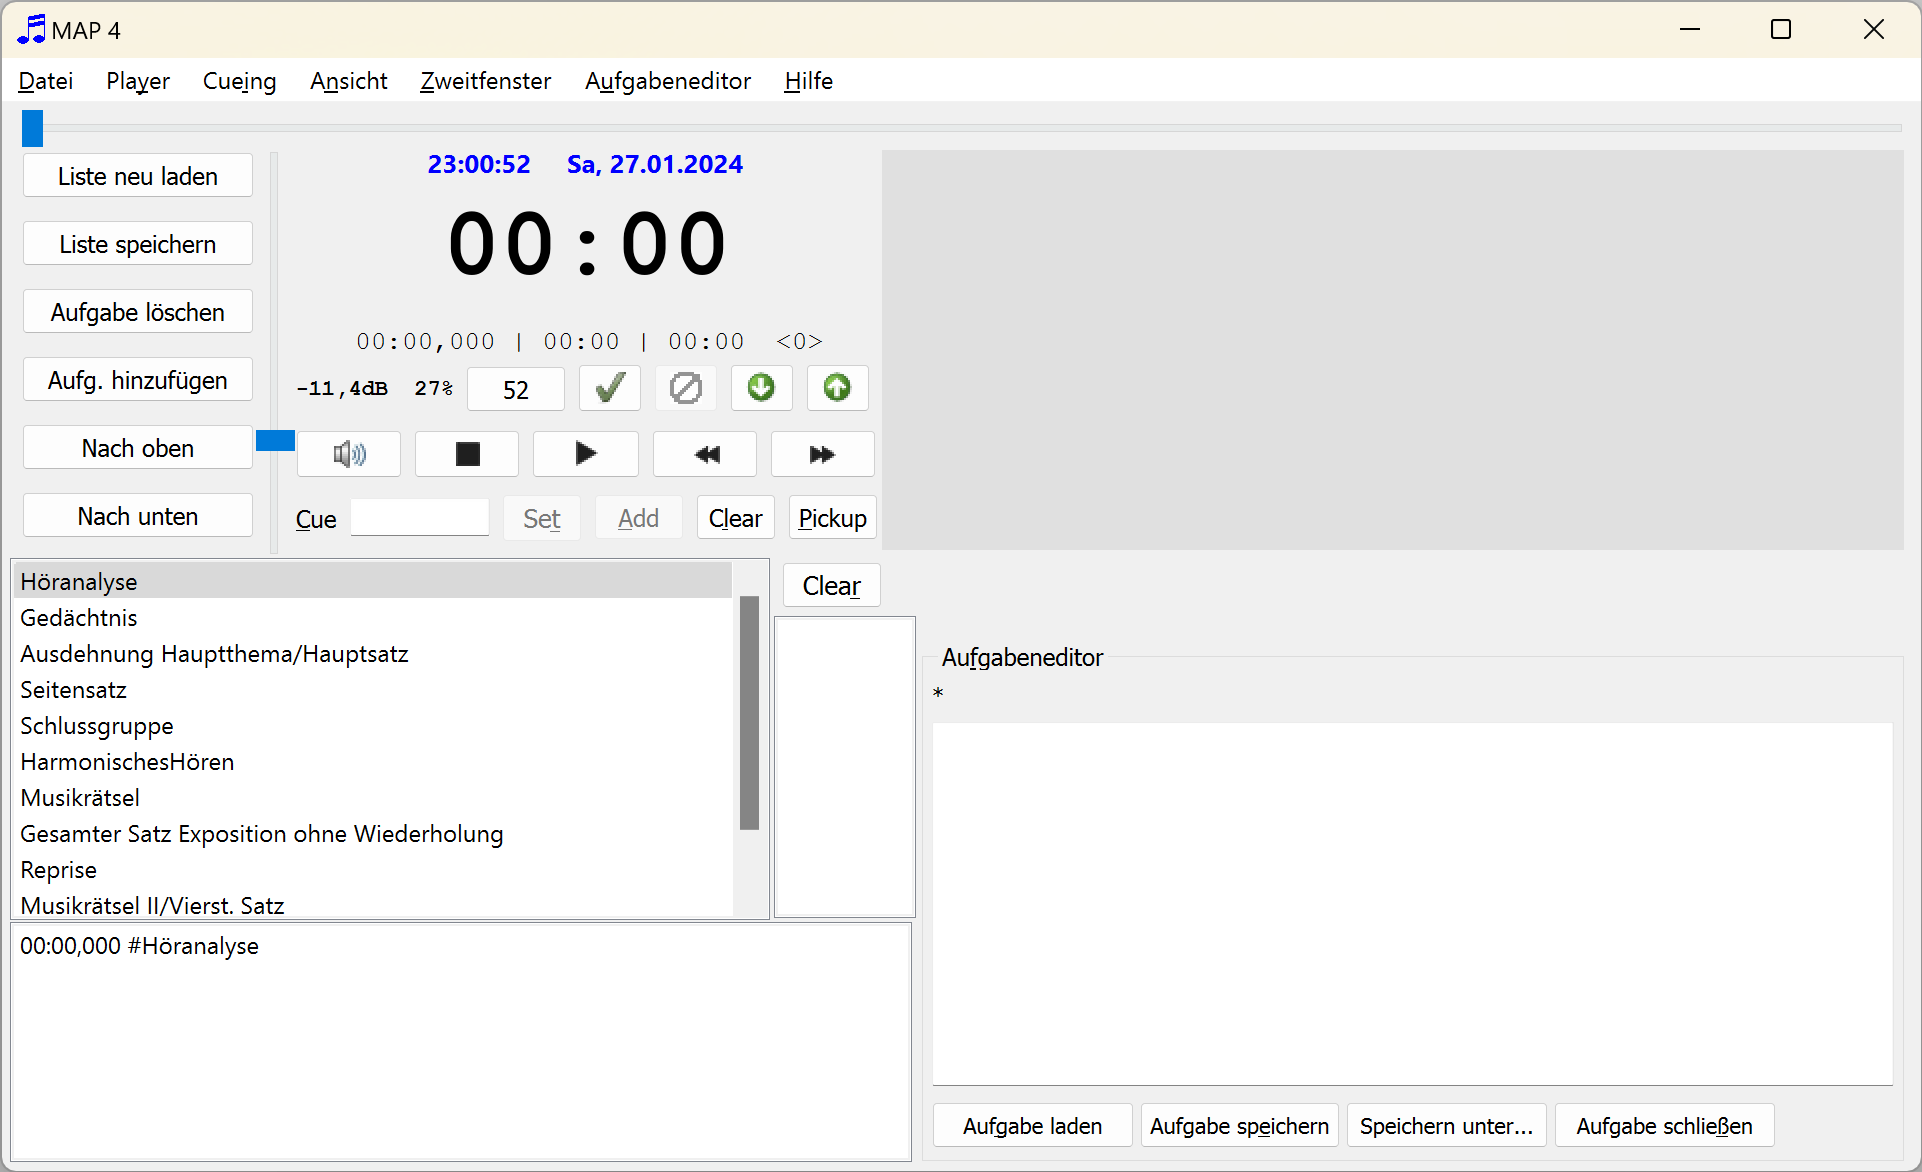
\includegraphics{/Users/manfreddings/Dropbox/QT/Map/Hilfe/Programmfenster.png}
\caption{Programmfenster}
\end{figure}

Die Aufgabendateien wiederum enthalten einen Aufgabentitel, den
relativen Pfad zu einer wav- oder mp3-Datei sowie optional Zeitmarken,
zu denen Hinweistexte im Programmfenster bzw. im Zweitfenster
dargestellt werden können. Ein Beispiel für eine Aufgabendatei:

{\scriptsize
	\begin{verbatim}
Klangbeispiel 1.1: Mozart, Quartett A-dur KV 464 I\#\twav\MozartQuartettAKV464IExposition.mp3
0#<h1>Themen/Themenfreie Abschnitte</h1><p>Fest und locker gefügtl</p><ul><li>Motive?</li></ul>
\end{verbatim}
}

Der erste Eintrag in der ersten Zeile bildet die Beschreibung der
Aufgabe, die im Programm in der Liste dargestellt wird. Nach dem
Trennzeichen \# steht der relative Pfad zur Mediendatei. Sie kann im
selben Verzeichnis wie die Aufgabenliste liegen oder - wie im Beispiel -
in einem Unterverzeichnis.

Alle weiteren Zeilen blenden zu einem gegeben Zeitpunkt (im Beispiel 0
Sekunden) den nachfolgend gegebenen Text ein. Dieser Text ist
vorzugsweise in HTML formuliert (hier also mit einer Überschrift, einem
Absatz und einer Aufzählungliste mit einem Aufzählungspunkt).

Alle Dateien sind reine Textdateien und können in jedem beliebigen
Texteditor erstellt und bearbeitet werden, Aufgabendateien auch im
internen \protect\hyperlink{BefehleImMenuAufgabeneditor}{Aufgabeneditor}
rechts im Programmfenster.

Aufgabendateien werden mit den einschlägigen Schaltflächen bzw. Befehlen
im Menü \protect\hyperlink{BefehleImMenuPlayer}{Player} abgespielt,
pausiert oder angehalten. Zudem lassen sich Cueing-Marken setzen, also
Zeitmarken, von denen aus die Sounddateien gestartet ewerden können.
Auch die Wiedergabelautstärke lässt sich einstellen sowie ein
automatisches Fading vornehmen.

Mit den Befehlen im Menü \protect\hyperlink{BefehleImMenuCueing}{Cueing}
lassen sich Zeitmarken setzen und ansteuern. Diese Zeitmarken sind
unabhängig von der gerade geladenen Aufgabenliste bzw. Aufgabe.

\hypertarget{menuxfcbefehle}{%
\section{Menübefehle}\label{menuxfcbefehle}}

\hypertarget{befehle-im-menuxfc-datei}{%
\subsection{Befehle im Menü Datei}\label{befehle-im-menuxfc-datei}}

\hypertarget{aufgabenliste-laden-strgf2}{%
\subsubsection{Aufgabenliste laden
(Strg+F2)}\label{aufgabenliste-laden-strgf2}}

Mit diesem Befehl öffnen sie eine vorhandene
\protect\hyperlink{aufgabenlisten}{Aufgabenliste}. Die vorhandene Datei
wird ohne Nachfrage geschlossen. Das gleiche bewirkt der Button \texttt{Liste\ neu\ laden}.

Eine Aufgabenliste kann auch per Drag and Drop aus dem Windows-Explorer
heraus auf das Programmfenster gezogen werden und wird dann genauso
geladen, wie wenn sie mit dem Befehl
\protect\hyperlink{AufgabeHinzufuegen}{Aufgabe hinzufügen} geladen
worden wäre.

\hypertarget{aufgabenliste-neu-laden}{%
\subsubsection{Aufgabenliste neu laden}\label{aufgabenliste-neu-laden}}

Mit diesem Befehl wird die aktuell geladene
\protect\hyperlink{aufgabenlisten}{Aufgabenliste} neu geladen. Dies ist
beispielsweise dann sinnvoll, wenn
\protect\hyperlink{aufgabendateien}{Aufgabendateien} mit einem externen
Editor oder dem internen
\protect\hyperlink{BefehleImMenuAufgabeneditor}{Aufgabeneditor}
verändert wurden.

Erst nach dem Neueinlesen werden die Änderungen in den veränderten
\protect\hyperlink{aufgabendateien}{Aufgabendateien} übernommen.

\hypertarget{aufgabenliste-speichern-umschf2}{%
\subsubsection{Aufgabenliste speichern
(Umsch+F2)}\label{aufgabenliste-speichern-umschf2}}

Dieser Befehl speichert die aktuell geöffnete
\protect\hyperlink{aufgabenlisten}{Aufgabenliste}. Das gleiche bewirkt
der Button \texttt{Liste\ speichern}.

\hypertarget{aufgabenliste-speichern-als}{%
\subsubsection{Aufgabenliste speichern
als...}\label{aufgabenliste-speichern-als}}

Dieser Befehl speichert die aktuell geladene
\protect\hyperlink{aufgabenlisten}{Aufgabenliste} unter einem anderen
Dateinamen.

\hypertarget{leere-aufgabenliste}{%
\subsubsection{Leere Aufgabenliste}\label{leere-aufgabenliste}}

Dieser Befehl schließt eine vorhandene
\protect\hyperlink{aufgabenlisten}{Aufgabenliste} ohne Nachfrage, legt
eine neue an und öffnet einen Dialog zur Vergabe eines Dateinamens. Die Aufgabenliste ist anschließend leer, bis
\protect\hyperlink{aufgabendateien}{Aufgabendateien} hinzugefügt werden.

\hypertarget{aufgabe-luxf6schen-entf}{%
\subsubsection{Aufgabe löschen (Entf)}\label{aufgabe-luxf6schen-entf}}

Dieser Befehl löscht die aktuell marktierte bzw. abgespielte
Aufgabendatei aus der Aufgabenliste. Die Liste ist anschließend
ungesichert und muss bei Bedarf gespeichert werden. Das gleiche bewirkt der Button \texttt{Aufgabe\ löschen}.

\hypertarget{aufgabe-nach-oben-strgumschhoch}{%
\subsubsection{Aufgabe nach oben
(Strg+Umsch+Hoch)}\label{aufgabe-nach-oben-strgumschhoch}}

Mit diesem Befehl wird die aktuell markierte und verwendete Aufgabe in
der \protect\hyperlink{aufgabenlisten}{Aufgabenliste} aufwärts
verschoben. Das gleiche bewirkt der Button \texttt{Nach\ oben}. Die
Aufgabenliste ist dadurch verändert und muss manuell
\protect\hyperlink{AufgabenlisteSpeichern}{gespeichert} werden.

\hypertarget{aufgabe-nach-unten-strgumschherunter}{%
\subsubsection{Aufgabe nach unten
(Strg+Umsch+Herunter)}\label{aufgabe-nach-unten-strgumschherunter}}

Mit diesem Befehl wird die aktuell markierte und verwendete Aufgabe in
der \protect\hyperlink{aufgabenlisten}{Aufgabenliste} aubärts
verschoben. Das gleiche bewirkt der Button \texttt{Nach\ unten}. Die
Aufgabenliste ist dadurch verändert und muss manuell
\protect\hyperlink{AufgabenlisteSpeichern}{gespeichert} werden.

\hypertarget{aufgabe-hinzufuxfcgen}{%
\subsubsection{Aufgabe hinzufügen}\label{aufgabe-hinzufuxfcgen}}

Dieser Befehl ruft einen Dateiauswahldialog auf, in dem Sie eine
bestehende \protect\hyperlink{Aufgabendatei}{Aufgabendatei} auswählen
können. Diese wird der aktuell geladenen Aufgabenliste am Ende angefügt.
Das gleiche bewirkt der Button \texttt{Aufg.\ hinzufügen}. Die
\protect\hyperlink{Aufgabenliste}{Aufgabenliste} ist dadurch verändert
und muss manuell \protect\hyperlink{AufgabenlisteSpeichern}{gespeichert}
werden. Eine \protect\hyperlink{Aufgabendatei}{Aufgabendatei} kann auch per Drag
and Drop aus dem Dateimanager heraus auf das Programmfenster gezogen
werden und wird dann genauso zur
\protect\hyperlink{Aufgabenliste}{Aufgabenliste} hinzugefügt, wie wenn
sie mit dem Befehl \texttt{Aufgabe\ hinzufügen} geladen worden wäre.

\hypertarget{aufgabenliste-bearbeiten}{%
\subsubsection{Aufgabenliste
bearbeiten}\label{aufgabenliste-bearbeiten}}

Dieser Befehl ruft den auf Ihrem Betriebssystem eingerichteten
Standardeditor mit der aktuell geladenen
\protect\hyperlink{aufgabenlisten}{Aufgabenliste} auf, welche auf diese
Weise manuell editiert werden kann.

\hypertarget{aufgabe-bearbeiten}{%
\subsubsection{Aufgabe bearbeiten}\label{aufgabe-bearbeiten}}

Dieser Befehl ruft den auf Ihrem Betriebssystem eingerichteten
Standardeditor mit der Datei der aktuell marktierten
\protect\hyperlink{ux5cux23Aufgabendatei}{Aufgabe} auf, welche auf diese
Weise manuell editiert werden kann. Alternativ können Aufgaben auch mit
dem \protect\hyperlink{BefehleImMenuAufgabeneditor}{programmeigenen
Editor} bearbeitet werden.

\hypertarget{in-explorer-zeigen}{%
\subsubsection{In Explorer zeigen}\label{in-explorer-zeigen}}

Dieser Befehl öffnet den Explorer mit dem Verzeichnis und der Ansicht
der gerade aktiven (markierten, abgespielten)
\protect\hyperlink{ux5cux23Aufgabendatei}{Aufgabendatei}).

\hypertarget{beenden-f4}{%
\subsubsection{Beenden (F4)}\label{beenden-f4}}

Dieser Befehl beendet MAP sofort. Es erfolgt keine Nachfrage, ob
ungesicherte Dateien (Aufgabenliste, Aufgaben) gespeichert werden
sollen.

\hypertarget{befehle-im-menuxfc-player}{%
\subsection{Befehle im Menü Player}\label{befehle-im-menuxfc-player}}

\hypertarget{play-bzw-pause-strgleertaste}{%
\subsubsection{Play bzw. Pause
(Strg+Leertaste)}\label{play-bzw-pause-strgleertaste}}

Dies startet die Wiedergabe der Audiodatei aus der aktuell ausgewählten
\protect\hyperlink{aufgabendateien}{Aufgabe}. Dadurch wandelt sich der
Menübefehl in den Befehl Pause und umgekehrt. Den gleichen Effekt
erreicht man auch durch Betätigen des Buttons im Player.

\hypertarget{stop-strgs}{%
\subsubsection{Stop (Strg+S)}\label{stop-strgs}}

Dies beendet die Wiedergabe der
\protect\hyperlink{FormatSounddateien}{Audiodatei} aus der aktuell
ausgewählten Aufgabe. Den gleichen Effekt erreicht man auch durch
Betätigen des Stop-Buttons im Player.

\hypertarget{vor-strgn-bzw-zuruxfcck-strgb}{%
\subsubsection{Vor (Strg+N) bzw. Zurück
(Strg+B)}\label{vor-strgn-bzw-zuruxfcck-strgb}}

Dies ruft die nächste bzw. vorherige
\protect\hyperlink{aufgabendateien}{Aufgabe} der aktuell geladenen
\protect\hyperlink{aufgabenlisten}{Aufgabeliste} auf.

\hypertarget{nuxe4chste-teilaufgabe-strgumschn-bzw-vorherige-teilaufgabe-strgumschb}{%
\subsubsection{Nächste Teilaufgabe (Strg+Umsch+N) bzw. vorherige
Teilaufgabe
(Strg+Umsch+B)}\label{nuxe4chste-teilaufgabe-strgumschn-bzw-vorherige-teilaufgabe-strgumschb}}

Bei \protect\hyperlink{aufgabendateien}{Aufgaben} mit Zeitmarkierungen
(quasi Teilaufgaben) springt dies die Zeitmarkierung nach bzw. vor der
aktuellen an. Sofern der Player im Stop- oder Pause-Modus ist, wird
lediglich die Zeitmarkierung angesprungen. Läuft eine Wiedergabe, so
springt diese unmittelbar an die Zeitmarke.

\hypertarget{lauter-strg--bzw-leiser-strg--}{%
\subsubsection{Lauter (Strg+ +) bzw. Leiser (Strg+
-)}\label{lauter-strg--bzw-leiser-strg--}}

Erhöhet bzw. senkt die Lautstärke der Wiedergabe

\hypertarget{fade-in-strgi}{%
\subsubsection{Fade in (Strg+I)}\label{fade-in-strgi}}

Setzt die Wiedergabelautstärke auf die Standardlautstärke. Der Befehl
ist nur wählbar, wenn zuvor ein \protect\hyperlink{FadeOut}{Fade out}
eingeleitet wurde.

\hypertarget{fade-out-strgf}{%
\subsubsection{Fade out (Strg+F)}\label{fade-out-strgf}}

Blendet die laufende Wiedergabe aus, wodurch der Lautstärkeregler auf 0
gefahren wird. Der Befehl ist nur anwählbar, wenn die
Wiedergabelautstärke nicht auf 0\% steht.

\hypertarget{fading-anhalten-strgh}{%
\subsubsection{Fading anhalten (Strg+H)}\label{fading-anhalten-strgh}}

Damit wird ein laufender Fadingprozess (\protect\hyperlink{FadeIn}{Fade
in} oder \protect\hyperlink{FadeOut}{out}) angehalten. Der Befehl steht
nur dann zur Verfügung, wenn zuvor ein Fading eingeleitet worden und
noch nicht abgeschlossen ist.

\hypertarget{standardvolume-festlegen-strgv}{%
\subsubsection{Standardvolume festlegen
(Strg+V)}\label{standardvolume-festlegen-strgv}}

Damit wird der Wiedergabepegel festgelegt, zu dem ein
\protect\hyperlink{FadeIn}{Fade in} erfolgen soll. Es wird der gerade
eingestellte Pegel verwendet.

\hypertarget{standardvolumen-anwenden-strg-}{%
\subsubsection{Standardvolumen anwenden (Strg+
\#)}\label{standardvolumen-anwenden-strg-}}

Damit wird der Wiedergabepegel auf den festgelegten
\protect\hyperlink{StandardvolumeFestlegen}{Standardpegel} eingestellt.

\hypertarget{mute-strg-m}{%
\subsubsection{Mute (Strg+ M)}\label{mute-strg-m}}

Stummschaltung oder Aufhebung der Stummschaltung, unterbindet die
Weiterleitung des Signals an die Ausgabe, unabhängig vom
Wiedergabezustand des Players.

\hypertarget{ganzton-huxf6her--ganzton-tiefer-f8-f12}{%
\subsubsection{Ganzton höher .. Ganzton tiefer
(F8-F12)}\label{ganzton-huxf6her--ganzton-tiefer-f8-f12}}

Damit wird die Wiedergabe beschleunigt oder abgebremst, was mit einer
Tonhöhenänderung verbunden ist.  Für jeden Befehl sind Tastenkürzel definiert:

\begin{itemize*}
\item
  Ganzton höher (F12)
\item
  Halbton höher (F11)
\item
  Normales Tempo (F10)
\item
  Ganzton tiefer (F9)
\item
  Halbton tiefer (F8)
\end{itemize*}

\hypertarget{befehle-im-menuxfc-cueing}{%
\subsection{Befehle im Menü Cueing}\label{befehle-im-menuxfc-cueing}}

\hypertarget{zu-cuingpoint-gehen-umschleertaste}{%
\subsubsection{Zu Cuingpoint gehen
(Umsch+Leertaste)}\label{zu-cuingpoint-gehen-umschleertaste}}

Damit wird die Wiedergabeposition auf die Zeit gesetzt, welche im
Eingabefeld \protect\hyperlink{EingabefeldCue}{Cue} vorgemerkt ist. Der
Befehl kann nur dann angewendet werden, wenn dort ein gültiger Zeitpunkt
angegeben ist.

\hypertarget{pickup-strgumschleertaste}{%
\subsubsection{Pickup
(Strg+Umsch+Leertaste)}\label{pickup-strgumschleertaste}}

Damit wird die aktuelle Wiedergabeposition in das
\protect\hyperlink{EingabefeldCue}{Eingabefeld Cue} eingetragen sowie
der \protect\hyperlink{Cuingliste}{Cuingliste} hinzugefügt.

\hypertarget{liste-luxf6schen}{%
\subsubsection{Liste Löschen}\label{liste-luxf6schen}}

Dies löschte die \protect\hyperlink{Cuingliste}{Cuingliste}.

\hypertarget{aufgabenliste-laden-f2}{%
\subsubsection{Aufgabenliste laden (F2)}\label{aufgabenliste-laden-f2}}

Mit diesem Befehl öffnen sie eine vorhandene
\protect\hyperlink{Aufgabenliste}{Aufgabenliste}. Die vorhandene Datei
wird ohne Nachfrage geschlossen.\\
Das gleiche bewirkt der Button Liste neu laden.

Eine Aufgabenliste kann auch per Drag and Drop aus dem Dateimanager
heraus auf das Programmfenster gezogen werden und wird dann genauso
geladen, wie wenn sie mit dem Befehl Aufgabe hinzufügen geladen worden
wäre.

\hypertarget{befehle-im-menuxfc-ansicht}{%
\subsection{Befehle im Menü Ansicht}\label{befehle-im-menuxfc-ansicht}}

\hypertarget{menuxfcleiste-esc}{%
\subsubsection{Menüleiste (Esc)}\label{menuxfcleiste-esc}}

Dies blendet die Menüleiste aus. Vorsicht: Die Menüleiste lässt sich
anschließend nur über den Tastaturbefehl (\texttt{Esc}-Taste) wieder
einblenden oder über das Kontextmenü, das mit der sekundären Maustaste
(also meist der rechten) eingeblendet werden kann.

\hypertarget{statusleite-umschesc}{%
\subsubsection{Statusleite (Umsch+Esc)}\label{statusleite-umschesc}}

Blendet die Statusleiste unten im Programmfenster ein- oder aus.

\hypertarget{audiodateiinfos-zeigen-f6}{%
\subsubsection{Audiodateiinfos zeigen
(F6)}\label{audiodateiinfos-zeigen-f6}}

Dies blendet in der Statusleiste den Pfad zur Audiodatei ein bzw. aus,
welche der ausgewählten \protect\hyperlink{aufgabendateien}{Aufgabe}
zugehörig ist.

\hypertarget{aufgabendateiinfos-zeigen-umschf6}{%
\subsubsection{Aufgabendateiinfos zeigen
(Umsch+F6)}\label{aufgabendateiinfos-zeigen-umschf6}}

Dies blendet in der Statusleiste den Pfad zur
\protect\hyperlink{aufgabendateien}{Aufgabendatei} ein bzw. aus, welche
der ausgewählten Aufgabe zugehörig ist.

\hypertarget{aufgabendetails-zeigen-strgf6}{%
\subsubsection{Aufgabendetails zeigen
(Strg+F6)}\label{aufgabendetails-zeigen-strgf6}}

Dies blendet die Liste mit den Detailinformationen zur aktuell geladenen
gewählten Aufgabe ein bzw. aus.

\hypertarget{kommentare-zeigen-strgk}{%
\subsubsection{Kommentare zeigen
(Strg+K)}\label{kommentare-zeigen-strgk}}

Dies blendet die Anzeige von Kommentaren ein bzw. aus, welche in der
aktuell wiedergegebenen
\protect\hyperlink{aufgabendateien}{Aufgabendatei} hinterlegt wurden.
Kommentare werden nur angezeigt, wenn die Wiedergabe aktiv ist bzw.
pausiert, nicht, wenn sie gestoppt ist.

\hypertarget{mit-zweitfenster-synchronisieren-strgf3}{%
\subsubsection{Mit Zweitfenster synchronisieren
(Strg+F3)}\label{mit-zweitfenster-synchronisieren-strgf3}}

Dies synchronisiert die Größe der Anzeige der Aufgabeninformationen mit
der des Zweitfensters (Popupfensters). Ist die Option nicht ausgewählt,
wird passt sich die Größe dem Programmfenster an.

\hypertarget{normalansicht-strgumscha}{%
\subsubsection{Normalansicht
(Strg+Umsch+A)}\label{normalansicht-strgumscha}}

Setzt die Fenstergröße auf eine vorgegebene, sinnvolle Größe, die alle
benötigten Elemente darstellt.

\hypertarget{lektionsansicht-strgumschl}{%
\subsubsection{Lektionsansicht
(Strg+Umsch+L)}\label{lektionsansicht-strgumschl}}

Die setzt die Fenstergröße auf eine kleinere Höhe, die insbesondere die
Anzeige der Aufgabendetails ausblendet. Dies ist sinnvoll, wenn
lediglich ein Bildschirm verwendet wird und bestimmte Informationen zur
aktuellen Aufgabe vor dem Auditorium verborgen bleiben sollen.

\hypertarget{leinwand-luxf6schen-strgl}{%
\subsubsection{Leinwand löschen
(Strg+L)}\label{leinwand-luxf6schen-strgl}}

Wenn der Player pausiert, werden mit diesem Befehl die der aktuellen
Wiedergabeposition zugeordneten Detailinformationen zur Aufgabe
ausgeblendet. Bei Fortsetzung der Wiedergabe erscheinen sie erneut. In
der Stoppposition des Players verschwinden sie abhängig vom Status des
Menübefehls \protect\hyperlink{BeiStopLeinwandLoeschen}{Bei Stop
Leinwand löschen (F4)} (oder bleiben ggf. erhalten).

\hypertarget{bei-stop-leinwand-luxf6schen-f4}{%
\subsubsection{Bei Stop Leinwand löschen
(F4)}\label{bei-stop-leinwand-luxf6schen-f4}}

Wenn dieser Menübefehl aktiviert ist (angehakt), so bleibt der bei der
letzten Wiedergabe dargestellte Detailtext zu einer Aufgabe erhalten.
Möchte man dieses Verhalten vermeiden (leere Leinwand bei Stoppen des
Players), so kann dies mit dem Menübefehl oder \texttt{F4} umgeschaltet
werden.

\hypertarget{kein-aufgabentext-f7}{%
\subsubsection{Kein Aufgabentext (F7)}\label{kein-aufgabentext-f7}}

Dies blendet die Darstellung der Detailinformationen zur aktuell
laufenden Ausgabe ein oder aus.

\hypertarget{keine-stoppuhr-strgf7}{%
\subsubsection{Keine Stoppuhr (Strg+F7)}\label{keine-stoppuhr-strgf7}}

Dieses blendet die Uhrzeitangabe der laufenden Wiedergabe aus. Der
Anzeigetext zur Aufgabe bleibt erhalten.

\hypertarget{hfm-stile}{%
\subsubsection{Hfm-Stile}\label{hfm-stile}}

Dies schaltet Farben ein, die zu einem bestimmten Skin in den
Lehrveranstaltungen des Verfassers passen (gelber Hintergrund).

\hypertarget{windows-stil}{%
\subsubsection{Windows-Stil}\label{windows-stil}}

Dies schaltet das die Farbeinstellungen von Windows-Installation ein
bzw. aus.

\hypertarget{schriftart}{%
\subsubsection{Schriftart...}\label{schriftart}}

Dies ruft einen Schriftauswahldialog aus, mit dem sich der Font für die
Aufgabeninhalte festlegen lässt.

\hypertarget{befehle-im-menuxfc-zweitfenster}{%
\subsection{Befehle im Menü
Zweitfenster}\label{befehle-im-menuxfc-zweitfenster}}

Das Zweitfenster oder "`Popupfenster"' dient zur Darstellung der
Stoppuhr und der Aufgabeninhalte auf einem zweiten Monitor. Es zeigt die
gleichen Angaben, die auch im Hauptfenster erscheinen. Seine Größe und
Position können unabhängig vom Programmfenster festgelegt werden.
Insbesondere kann es auf einen zweiten Monitor bzw. den Beamer bewegt
werden.

\hypertarget{popupfenster-f3}{%
\subsubsection{Popupfenster (F3)}\label{popupfenster-f3}}

Dieser Befehl blendet das Zweitfenster ein- oder aus. Dass es
ausgeblendet ist, ist daran erkennbar, dass die Stoppuhr im Hauptfenster
in \emph{kursiver Schriftart} dargestellt wird.

\hypertarget{standardgruxf6uxdfe-f5}{%
\subsubsection{Standardgröße (F5)}\label{standardgruxf6uxdfe-f5}}

Dies verändert die Größe des Zweitfensters auf einen Standardwert.

\hypertarget{stoppuhransicht-abschalten-strgf5}{%
\subsubsection{Stoppuhransicht abschalten
(Strg+F5)}\label{stoppuhransicht-abschalten-strgf5}}

Dies schalte die Anzeige der Wiedergabezeit im Zweitfenster ein oder
aus.

\hypertarget{veruxe4nderung-der-gruxf6uxdfe-und-position-des-zweitfensters}{%
\subsubsection{Veränderung der Größe und Position des
Zweitfensters}\label{veruxe4nderung-der-gruxf6uxdfe-und-position-des-zweitfensters}}

Die geht umständlich über die nachfolgend genannten Menübefehle,
komfortabler jedoch per Tastenkombination.

\hypertarget{uxe4ndern-der-gruxf6uxdfe}{%
\paragraph{Ändern der Größe:}\label{uxe4ndern-der-gruxf6uxdfe}}

\begin{itemize}
\item
  Enger (Alt+links)
\item
  Weiter (Alt+rechts)
\item
  Kleiner (Alt+auf)
\item
  Größer(Alt+ab)
\end{itemize}

\hypertarget{uxe4ndern-der-position-fein-kleinschrittig}{%
\paragraph{Ändern der Position (fein,
kleinschrittig)}\label{uxe4ndern-der-position-fein-kleinschrittig}}

\begin{itemize}
\item
  Nach rechts (Strg+rechts)
\item
  Nach links (Strg+links)
\item
  Nach oben (Strg+auf)
\item
  Nach unten (Strg+ab)
\end{itemize}

\hypertarget{uxe4ndern-der-position-grob-schnell}{%
\paragraph{Ändern der Position (grob,
schnell)}\label{uxe4ndern-der-position-grob-schnell}}

\begin{itemize}
\item
  Schnell rechts (Alt+Umsch+rechts)
\item
  Schnell links (Alt+Umsch+links)
\item
  Schnell oben (Alt+Umsch+auf)
\item
  Schnell unten (Alt+Umsch+ab)
\end{itemize}

\hypertarget{fenster-zuruxfcckholen-strgruxfccktaste}{%
\subsubsection{Fenster zurückholen
(Strg+Rücktaste)}\label{fenster-zuruxfcckholen-strgruxfccktaste}}

Die befördert das Zweitfenster an die äußerste linke obere Position,
also auf den Hauptbildschirm zurück.

\hypertarget{hfm-stil}{%
\subsubsection{HfM-Stil}\label{hfm-stil}}

Schaltet unabhängig vom Stil des Hauptfensters die Farbauswahl des in
den Lehrveranstaltungen des Verfassers passenden Skins ein (gelber
Hintergrund).

\hypertarget{stil-des-hauptfensters}{%
\subsubsection{Stil des Hauptfensters}\label{stil-des-hauptfensters}}

Ist diese Option aktiviert, so übernimmt das Zweitfenster den im
Hauptfenster aktivierten Stil.

\hypertarget{befehle-im-menuxfc-aufgabeneditor}{%
\subsection{Befehle im Menü
Aufgabeneditor}\label{befehle-im-menuxfc-aufgabeneditor}}

Die Befehle dieses Menüs sind überwiegend auch über Schaltfläche im
Editorbereich erreichbar. Wird eine Aufgabe bearbeitet, so muss sie
anschließend unbedingt gespeichert werden. Dies geschieht nicht
automatisch. Auch beim Beenden des Programms wird im Falle einer
veränderten Datei \emph{nicht} zum Speichern aufgefordert. Änderungen
gehen daher möglicherweise verloren, wenn nicht manuell gespeichert
wurde.

Wurde eine Aufgabe verändert und gespeichert, wird die aktuell geladene
\protect\hyperlink{aufgabenlisten}{Aufgabenliste} \emph{nicht}
aktualisiert. Dies muss
\protect\hyperlink{AufgabenlisteNeuLaden}{manuell} erfolgen.

\hypertarget{editor-anzeigen-strge}{%
\subsubsection{Editor anzeigen (Strg+E)}\label{editor-anzeigen-strge}}

Dies blendet den programmeigenen Aufgabeneditor ein bzw. aus.

\hypertarget{aufgabe-in-editor-laden-strgl}{%
\subsubsection{Aufgabe in Editor laden
(Strg+L)}\label{aufgabe-in-editor-laden-strgl}}

Dies läd die aktuell ausgewählte Aufgabe in den Editor. Die gleiche
Wirkung hat die Schaltfläche \texttt{Aufgabe\ laden} im Editorbereich.
Dort kann sie wie in jedem üblichen Texteditor bearbeitet und
anschließend bei Bedarf
\protect\hyperlink{AufgabeSpeichern}{gespeichert} werden.

\hypertarget{aufgabe-speichern-strgumschs}{%
\subsubsection{Aufgabe speichern
(Strg+Umsch+S)}\label{aufgabe-speichern-strgumschs}}

Speichert die Änderungen an der aktuell im Aufgabeneditor geladenen
Aufgabe. Die gleiche Wirkung hat die Schaltfläche
\texttt{Aufgabe\ speichern} im Editorbereich.

\hypertarget{aufgabe-speichern-unter}{%
\subsubsection{Aufgabe speichern
unter...}\label{aufgabe-speichern-unter}}

Speichert die Änderungen an der aktuell im Aufgabeneditor geladenen
Aufgabe unter Abfrage eines neuen Dateinamens. Die Erweiterung für
\protect\hyperlink{aufgabendateien}{Aufgabendateien} muss \texttt{.auf}
sein.

Die gleiche Wirkung hat die Schaltfläche \texttt{Speichern\ unter...} im
Editorbereich.

\hypertarget{aufgabe-schlieuxdfen}{%
\subsubsection{Aufgabe schließen}\label{aufgabe-schlieuxdfen}}

Blendet eine im Editorbereich geladene Aufgabe wieder aus. Die gleiche
Wirkung hat die Schaltfläche \texttt{Aufgabe\ schließen} im
Editorbereich.

\hypertarget{befehle-im-menuxfc-hilfe}{%
\subsection{Befehle im Menü Hilfe}\label{befehle-im-menuxfc-hilfe}}

\hypertarget{hilfe-f1}{%
\subsubsection{Hilfe (F1)}\label{hilfe-f1}}

Ruft diese Online-Hilfe auf.

\hypertarget{internen-hilfebrowser-verwenden}{%
\subsubsection{Internen Hilfebrowser
verwenden}\label{internen-hilfebrowser-verwenden}}

Dies schaltet ein bzw. aus, dass die Hilfe-Datei über die programmeigene
Hilfefunktion dargestellt wird. Anderenfalls erfolgt die Darstellung
über das Standardprogramm, das im Betriebssystem konfiguriert wurde.

Schlägt letzteres - aus welchen Gründen auch immer - fehl, so wird stets
der interne Browser von MAP verwendet.

\hypertarget{uxfcber-map}{%
\subsubsection{Über MAP}\label{uxfcber-map}}

Ruft einen Dialog mit Informationen zum Programm und zur aktuellen
Version auf.

\hypertarget{die-programmoberfluxe4che}{%
\section{Die Programmoberfläche}\label{die-programmoberfluxe4che}}

Im Programmfenster ist ein Kontextmenü verfügbar (Klicken mit der
sekundären Maustaste).

Aufgabenlisten und Aufgabendateien können per Drag und Drop geladen
werden (aus dem Explorer in das Programmfenster ziehen).

Etliche Menübefehle können über Buttons erreicht werden. Wichtige
Funktionen sind über Schieberegler verfügbar:

\begin{itemize}
\item
  Die Lautstärke wird über den senkrechten Schieberegler links neben der
  Uhr eingestellt.
\item
  Die aktuelle Wiedergabeposition kann manuell über den horizontalen
  Schieberegler festgesetzt werden. Dieser zeigt auch die laufende
  Wiedergabeposition an.
\end{itemize}

\begin{figure}
\centering
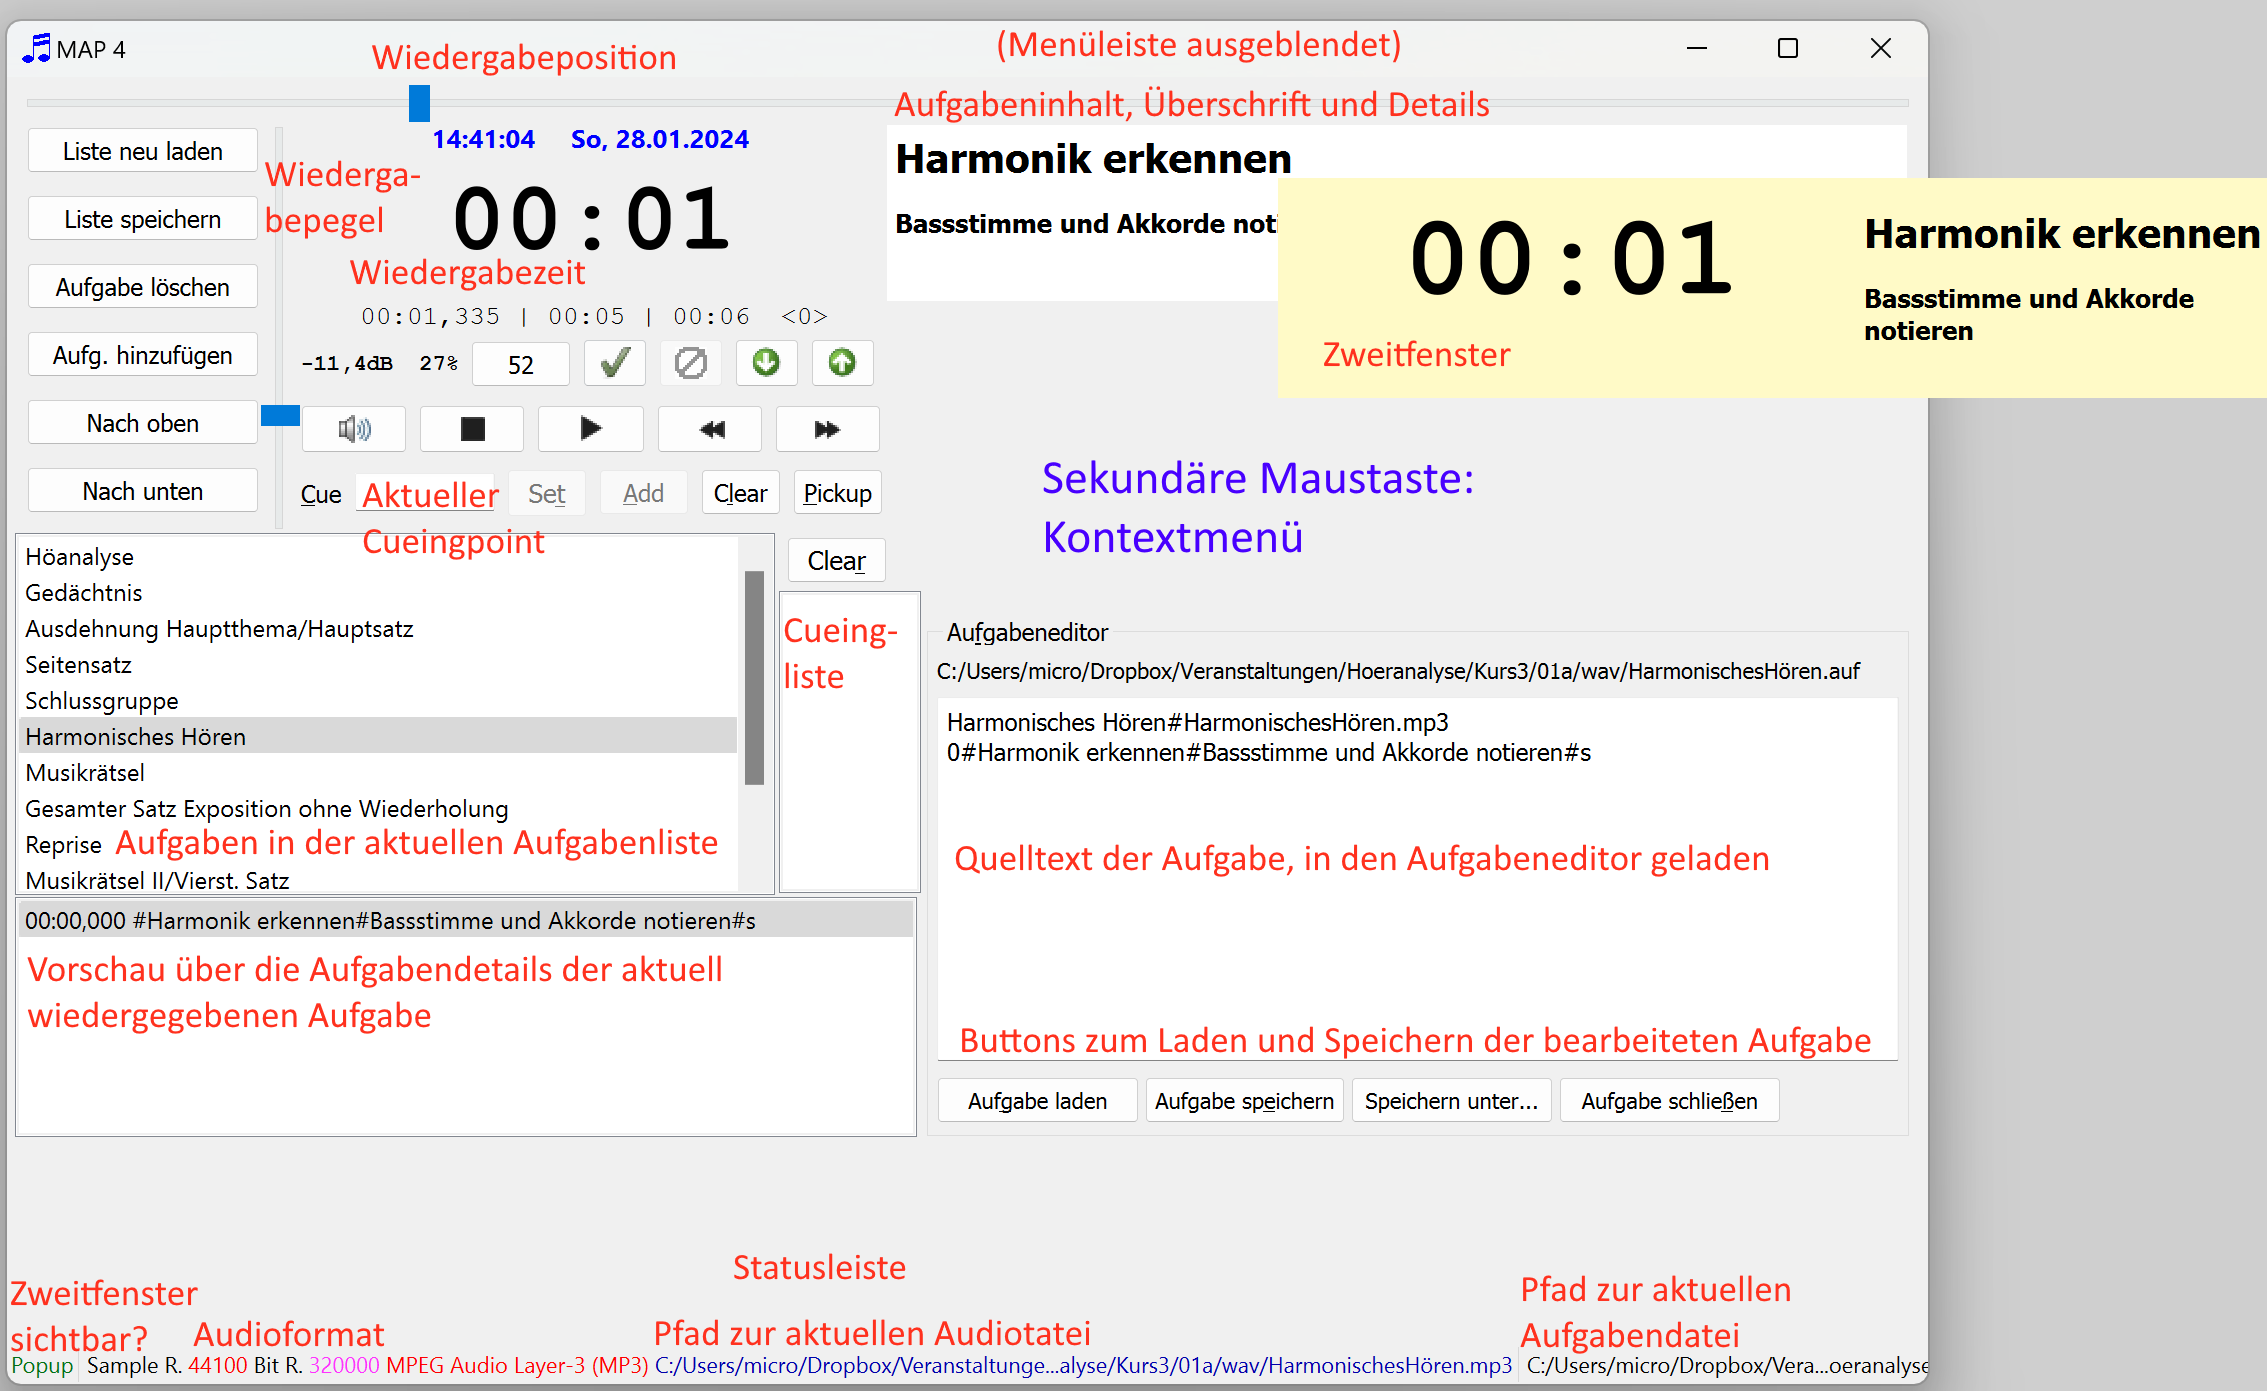
\includegraphics{/Users/manfreddings/Dropbox/QT/Map/Hilfe/Oberflaeche.png}
\caption{Oberflaeche}
\end{figure}

Die sekundäre Maustaste (meist also die rechte) ruft ein Kontextmenü
auf.

\hypertarget{das-eingabefeld-cue}{%
\subsubsection{Das Eingabefeld Cue}\label{das-eingabefeld-cue}}

Hier geben Sie einen Zeitpunkt ein, zu dem die Wiedergabeposition
springen soll. Das Format ist \texttt{mm:ss{[},xxx{]}} (z. B. 01:23 oder
\texttt{01:23,456}. Die Zehntel bis Tausendstelsekundenangabe ist
fakultativ. Neben der manuellen Eingabe kann auch ein Doppelklick auf
die Cuingliste erfolgen oder die Anwendung des Befehls
\protect\hyperlink{Pickup}{Pickup (Strg+Umsch+Leertaste)}.

\hypertarget{die-cuingliste}{%
\subsubsection{Die Cuingliste}\label{die-cuingliste}}

Hier lassen sich verschiedene Zeitpunkte (aufsteigend sortiert)
speichern, welche per Doppelklick in das
\protect\hyperlink{EingabefeldCue}{Cuing-Eingabefeld} geschrieben werden
können. Die Einträge können entweder

\begin{itemize}
\item
  mit dem Befehl \protect\hyperlink{Pickup}{Cuing\textbar Pickup
  (Strg+Umsch+Leertaste)} erfolgen,
\item
  über den Button \texttt{Pickup}
\item
  oder indem der aktuelle Eintrag im
  \protect\hyperlink{EingabefeldCue}{Cuing-Eingabefeld} über den Button
  Add in die Liste geschrieben wird.
\end{itemize}

Mit Hilfe der Taste \texttt{Entf} kann ein markierter Eintrag gelöscht
werden. Der Button \texttt{Clear} oberhalb der Liste leert diese
insgesamt.

\hypertarget{das-zweitfenster}{%
\subsection{Das Zweitfenster}\label{das-zweitfenster}}

Das Zweitfenster zeigt - je nach Einstellungen im Menü
\protect\hyperlink{BefehleImMenuAnsicht}{Ansicht} - die laufende
Zeitanzeige und Hinweistexte zur aktuell geladenen und abgespielten
\protect\hyperlink{Aufgabendatei}{Aufgabendatei}. Mit den Befehlen im
Menü \protect\hyperlink{BefehleImMenuZweitfenster}{Zweitfenster} kann es
ein-/bzw. ausgeblendet, verschoben und in der Größe angepasst werden.
Insbesondere lässt es sich auf einen Zweitbildschirm verschieben.

Das Zweitfenster wird als "`always on top"'-Fenster immer über allen
anderen Fenstern in Windows dargestellt und verdeckt somit darunter
befindliche Inhalte.

\hypertarget{anhang}{%
\section{Anhang}\label{anhang}}

\hypertarget{aufgabenlisten}{%
\subsection{Aufgabenlisten}\label{aufgabenlisten}}

Aufgabenlisten sind einfache Textdateien, welche eine Folge von
Aufgabendateien enthalten. Aufgabenlisten müssen die Erweiterung \computer{.afl}
besitzen. Pro Zeile verweisen sie auf eine Aufgabendatei, die sich im
selben Verzeichnis befinden muss, beispielsweise so:

\begin{Shaded}
\begin{Highlighting}[]
\NormalTok{aufgabe1.auf}
\NormalTok{aufgabe2.auf}
\NormalTok{aufgabe3.auf}
\end{Highlighting}
\end{Shaded}

Wenn die Datei geladen wird, erscheinen die Aufgaben im Hauptfenster und
können nacheinander abgespielt werden.

\hypertarget{aufgabendateien}{%
\subsection{Aufgabendateien}\label{aufgabendateien}}

Aufgabendateien sind einfache Textdateien, welche die Informationen über
die abzuspielende wav- oder mp3-Datei enthalten sowie optional
Zeitmarken definieren können, zu denen bestimmte Informationen angezeigt
werden können. Eine Aufgabendatei kann folgendermaßen aussehen:

\begin{Shaded}
\begin{Highlighting}[]
\NormalTok{Vier extrem bekannte Werke\#Musikrätsel extrem.mp3}
\NormalTok{0\#Vier extrem bekannte Werke\#Werk 1\#l}
\NormalTok{0:46\#Vier extrem bekannte Werke\#Werk 2\#l}
\NormalTok{1:32\#Vier extrem bekannte Werke\#Werk 3\#l}
\NormalTok{2:33\#Vier extrem bekannte Werke\#Werk 4\#l}
\end{Highlighting}
\end{Shaded}

In Zeile 1 befindet sich ein Titelhinweis, der in MAP angezeigt wird,
dann als Trennzeichen das \# und schließlich der Dateiname bzw. relative
Dateipfad der mp3 oder wav-Datei. Diese kann sich in einem beliebigen
Unterverzeichnis (allerdings nicht in einem übergeordneten Verzeichnis)
befinden. Im Beispiel oben liegt die abzuspielende Datei
\texttt{KlassikerDerModerne.mp3} im Unterverzeichnis \texttt{Medien}.

Die Mediendatei können beliebige wav-Files sein. Im Falle von mp3-Files
ist darauf zu achten, dass unter Windows eine korrekte Wiedergaben nur
gewährleistet ist, wenn das Format Layer-3, 44100 Hz, 320 kbps, stereo
verwendet wird. In den weiteren Zeilen befindet sich

\begin{itemize}
\item
  in der ersten Spalte ein Timecode, entweder als Sekunden oder als
  Minuten und Sekunden (mm:ss) mit optionalen Millisekunden (mm:ss,xxx),
\item
  das Trennzeichen (\#),
\item
  in der zweiten Spalte eine Überschrift
\item
  das Trennzeichen (\#),
\item
  ein Erläuterungstext. Dieser kann nach einem weiteren Trennzeichen
  (\#) und s, m oder l wie small, medium, large als mit kleiner,
  normaler oder großer Schriftart formatiert gekennzeichnet werden. Die
  Voreinstellung ist medium.
\item
  Optional kann nach zwei \%\% ein Kommentar folgen, der im
  Programmfenster unten ausgegeben wird.
\end{itemize}

Die Überschrift und der Erläuterungstext werden exakt dann ausgegeben,
wenn die Zeitangabe zu Beginn der Spalte erreicht ist.

\hypertarget{alternatives-format-fuxfcr-uxfcberschrift-und-erluxe4uterungen}{%
\subsubsection{Alternatives Format für Überschrift und
Erläuterungen}\label{alternatives-format-fuxfcr-uxfcberschrift-und-erluxe4uterungen}}

Alternativ kann nach der Zeitangabe auch html-Code stehen,
beispielsweise\\
{\footnotesize
\texttt{00:10,123\#\textless{}h1\textgreater{}Überschrift\textless{}/h1\textgreater{}\textless{}h2\textgreater{}Unterüberschrift\textless{}/h2\textgreater{}\textless{}p\textgreater{}Erläuterungstext\textless{}/p\textgreater{}\%\%Kommentar}}

\hypertarget{format-der-sounddateien}{%
\subsection{Format der Sounddateien}\label{format-der-sounddateien}}

Wave-Dateien werden unter Windows und Linux korrekt wiedergegeben.
Sollen mp3-Files zum Einsatz kommen, so werden sie unter Windows in
Abhängigkeit von den installierten Codices und der Betriebssystemversion
unter Umständen fehlerhaft wiedergegeben. Insbesondere sind Zeitangaben
und -markieren fehlerhaft. Dies lässt sich vermeiden, wenn mp3 - Dateien folgendes Format haben:\\
\texttt{Layer-3,\ 44100\ Hz,\ 320\ kbps,\ stereo}

\hypertarget{lizenz}{%
\subsection{Lesser General Public License}\label{lizenz}}

This program is free software; you can redistribute it and/or modify it
under the terms of the LGP Lesser General Public License as published by
the Free Software Foundation; either version 3 of the License, or (at
your option) any later version.\\
This program is distributed in the hope that it will be useful, but
WITHOUT ANY WARRANTY; without even the implied warranty of
MERCHANTABILITY or FITNESS FOR A PARTICULAR PURPOSE.\\
You should have received a copy of the GNU General Public License along
with this program; if not, write to:\\
Free Software Foundation, Inc.\\
51 Franklin Street, Suite 500\\
Boston, MA 02110-1335, USA.

\url{www.fsf.org}

GNU LESSER GENERAL PUBLIC LICENSE

Version 3, 29 June 2007

Copyright © 2007 Free Software Foundation, Inc. \url{http://fsf.org/}

Everyone is permitted to copy and distribute verbatim copies of this
license document, but changing it is not allowed.

This version of the GNU Lesser General Public License incorporates the
terms and conditions of version 3 of the GNU General Public License,
supplemented by the additional permissions listed below.

\begin{enumerate}
\def\labelenumi{\arabic{enumi}.}
\item
  Additional Definitions.
\end{enumerate}

As used herein, ``this License'' refers to version 3 of the GNU Lesser
General Public License, and the ``GNU GPL'' refers to version 3 of the
GNU General Public License.

``The Library'' refers to a covered work governed by this License, other
than an Application or a Combined Work as defined below.

An ``Application'' is any work that makes use of an interface provided
by the Library, but which is not otherwise based on the Library.
Defining a subclass of a class defined by the Library is deemed a mode
of using an interface provided by the Library.

A ``Combined Work'' is a work produced by combining or linking an
Application with the Library. The particular version of the Library with
which the Combined Work was made is also called the ``Linked Version''.

The ``Minimal Corresponding Source'' for a Combined Work means the
Corresponding Source for the Combined Work, excluding any source code
for portions of the Combined Work that, considered in isolation, are
based on the Application, and not on the Linked Version.

The ``Corresponding Application Code'' for a Combined Work means the
object code and/or source code for the Application, including any data
and utility programs needed for reproducing the Combined Work from the
Application, but excluding the System Libraries of the Combined Work.

\begin{enumerate}
\def\labelenumi{\arabic{enumi}.}
\item
  Exception to Section 3 of the GNU GPL.
\end{enumerate}

You may convey a covered work under sections 3 and 4 of this License
without being bound by section 3 of the GNU GPL.

\begin{enumerate}
\def\labelenumi{\arabic{enumi}.}
\item
  Conveying Modified Versions.
\end{enumerate}

If you modify a copy of the Library, and, in your modifications, a
facility refers to a function or data to be supplied by an Application
that uses the facility (other than as an argument passed when the
facility is invoked), then you may convey a copy of the modified
version:

\NormalTok{a) under this License, provided that you make a good faith effort to ensure that, in the event an Application does not supply the function or data, the facility still operates, and performs whatever part of its purpose remains meaningful, or}
\NormalTok{b) under the GNU GPL, with none of the additional permissions of this License applicable to that copy.}

\begin{enumerate}
\def\labelenumi{\arabic{enumi}.}
\item
  Object Code Incorporating Material from Library Header Files.
\end{enumerate}

The object code form of an Application may incorporate material from a
header file that is part of the Library. You may convey such object code
under terms of your choice, provided that, if the incorporated material
is not limited to numerical parameters, data structure layouts and
accessors, or small macros, inline functions and templates (ten or fewer
lines in length), you do both of the following:


\NormalTok{a) Give prominent notice with each copy of the object code that the Library is used in it and that the Library and its use are covered by this License.}
\NormalTok{b) Accompany the object code with a copy of the GNU GPL and this license document.}


\begin{enumerate}
\def\labelenumi{\arabic{enumi}.}
\item
  Combined Works.
\end{enumerate}

You may convey a Combined Work under terms of your choice that, taken
together, effectively do not restrict modification of the portions of
the Library contained in the Combined Work and reverse engineering for
debugging such modifications, if you also do each of the following:

\NormalTok{a) Give prominent notice with each copy of the Combined Work that the Library is used in it and that the Library and its use are covered by this License.}
\NormalTok{b) Accompany the Combined Work with a copy of the GNU GPL and this license document.}
\NormalTok{c) For a Combined Work that displays copyright notices during execution, include the copyright notice for the Library among these notices, as well as a reference directing the user to the copies of the GNU GPL and this license document.}
\NormalTok{d) Do one of the following:}
\NormalTok{    0) Convey the Minimal Corresponding Source under the terms of this License, and the Corresponding Application Code in a form suitable for, and under terms that permit, the user to recombine or relink the Application with a modified version of the Linked Version to produce a modified Combined Work, in the manner specified by section 6 of the GNU GPL for conveying Corresponding Source.}
\NormalTok{    1) Use a suitable shared library mechanism for linking with the Library. A suitable mechanism is one that (a) uses at run time a copy of the Library already present on the user\textquotesingle{}s computer system, and (b) will operate properly with a modified version of the Library that is interface{-}compatible with the Linked Version.}
\NormalTok{e) Provide Installation Information, but only if you would otherwise be required to provide such information under section 6 of the GNU GPL, and only to the extent that such information is necessary to install and execute a modified version of the Combined Work produced by recombining or relinking the Application with a modified version of the Linked Version. (If you use option 4d0, the Installation Information must accompany the Minimal Corresponding Source and Corresponding Application Code. If you use option 4d1, you must provide the Installation Information in the manner specified by section 6 of the GNU GPL for conveying Corresponding Source.)}


\begin{enumerate}
\def\labelenumi{\arabic{enumi}.}
\item
  Combined Libraries.
\end{enumerate}

You may place library facilities that are a work based on the Library
side by side in a single library together with other library facilities
that are not Applications and are not covered by this License, and
convey such a combined library under terms of your choice, if you do
both of the following:


\NormalTok{a) Accompany the combined library with a copy of the same work based on the Library, uncombined with any other library facilities, conveyed under the terms of this License.}
\NormalTok{b) Give prominent notice with the combined library that part of it is a work based on the Library, and explaining where to find the accompanying uncombined form of the same work.}


\begin{enumerate}
\def\labelenumi{\arabic{enumi}.}
\item
  Revised Versions of the GNU Lesser General Public License.
\end{enumerate}

The Free Software Foundation may publish revised and/or new versions of
the GNU Lesser General Public License from time to time. Such new
versions will be similar in spirit to the present version, but may
differ in detail to address new problems or concerns.

Each version is given a distinguishing version number. If the Library as
you received it specifies that a certain numbered version of the GNU
Lesser General Public License ``or any later version'' applies to it,
you have the option of following the terms and conditions either of that
published version or of any later version published by the Free Software
Foundation. If the Library as you received it does not specify a version
number of the GNU Lesser General Public License, you may choose any
version of the GNU Lesser General Public License ever published by the
Free Software Foundation.

If the Library as you received it specifies that a proxy can decide
whether future versions of the GNU Lesser General Public License shall
apply, that proxy's public statement of acceptance of any version is
permanent authorization for you to choose that version for the Library.

\end{document}
